\documentclass{article}
\documentclass[10pt]{beamer}

\usetheme[progressbar=frametitle]{metropolis}
\usepackage{appendixnumberbeamer}
\usepackage[utf8]{inputenc}    
\usepackage{booktabs}
\usepackage[scale=2]{ccicons}

\usepackage{pgfplots}
\usepgfplotslibrary{dateplot}

\usepackage{xspace}
\newcommand{\themename}{\textbf{\textsc{metropolis}}\xspace}

\title{Memory span of recurrent neural nets}
\subtitle{Master Thesis}
% \date{\today}
\date{}
\author{Jaroslav Ištok}
%\institute{Faculty of Mathematics Physics and Informatics Comenius University Bratislava}
% \titlegraphic{\hfill\includegraphics[height=1.5cm]{logo.pdf}}

\begin{document}

\maketitle

\begin{frame}{Overview}
  \setbeamertemplate{section in toc}[sections numbered]
  \tableofcontents[hideallsubsections]
\end{frame}

\section{SOM}


\begin{frame}[fragile]{SOM}

\begin{itemize}
\item Self organizing map
\item Biologicaly motivated model
\item Unsupervised competitive learning
\item Clustering
\item Preserving topological features
\item Quantization error
\end{itemize}

Find Winner
\begin{equation*}
i^* = argmin_i||x-w_i|| 
\end{equation*}

Rule for update weights
\begin{equation*}
w_i(t+1) = w_i(t) + \alpha(t)h(i^*, i)([x(t) - w_i(t)]
\end{equation*}

\end{frame}

\section{Recurrent SOM}

\begin{frame}[fragile]{Recurrent SOM}
Self organizing map with context from previous steps
\begin{itemize}
\item RecSom - context is copy of whole map from previous step
\item Many attributes
\end{itemize}
Weights update
\begin{equation*}
w_i(t+1) = w_i(t) + zh_{ik}[s(t) - w_i(t)]
\end{equation*}
\begin{equation*}
c_i(t+1) = c_i(t) + zh_{ik}[y(t - 1) - c_i(t)]
\end{equation*}
\begin{equation*}
y_i=exp(-d_i)
\end{equation*}
Distance
\begin{equation*}
d_i(t) = \alpha||x(t)-w_i||^2 + \beta||r(t)-c_i||^2
\end{equation*}
Recursive context
\begin{equation*}
r(t)=[y_i(t-1),...,y_N(t-1)]
\end{equation*}
\end{frame}

\section{Merge SOM}

\begin{frame}[fragile]{Merge SOM}

\begin{itemize}
\item In Merge SOM \textbf{context is not} copy of whole map from previous step
\item Fewer parameters than RecSOM
\item $\gamma_1$ $\gamma_2$ - learning rates
\item $h_{\sigma}$ - Gaussian shaped function
\item $d_N$ - neighborhood function
\end{itemize}
Weights update
\begin{equation*}
\Delta w_i = \gamma_{1} \cdot h_{\sigma}(d_{N}(i, I_{t})) \cdot (x^t - w^i)
\end{equation*}
\begin{equation*}
\Delta c_i = \gamma_{2} \cdot h_{\sigma}(d_{N}(i, I_{t})) \cdot (c^t - c^i)
\end{equation*}

Distance
\begin{equation*}
d_i(t) = (1-\alpha) \cdot ||x^t - w^i||^2 + \alpha \cdot ||c^t - c^i||^2
\end{equation*}
Recursive context
\begin{equation*}
c^t = (1 - \beta) \cdot w^{I_{t-1}} + \beta \cdot c^{I_{t-1}}
\end{equation*}

\end{frame}

\section{SRN - Elman network}

\begin{frame}[fragile]{SRN - Elman network}

\begin{itemize}
\item Elman recurrent network
\item Training with backpropagation through time
\item Supervised learning
\item Context layer 
\end{itemize}

\end{frame}


\begin{frame}[fragile]{SRN - Elman network}

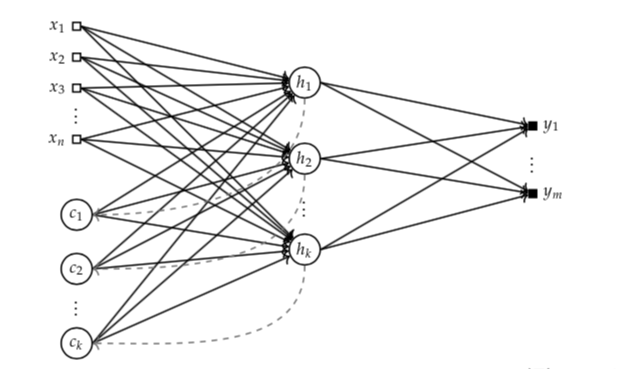
\includegraphics[width=\textwidth]{elman}

\end{frame}

\begin{frame}[fragile]{Measuring memory span}

\begin{itemize}
\item Words sequences
\item Every neuron will have set of letters
\item If this neuron is winner, it will save letter to its set of letters (receptive field)
\item Neuron saves $n$ previous letters in its receptive field
\item We can then find longest common sub-sequence and calculate weighted average
\item This will be our measure of memory span
\end{itemize}

\end{frame}

\begin{frame}[fragile]{Example of receptive field}
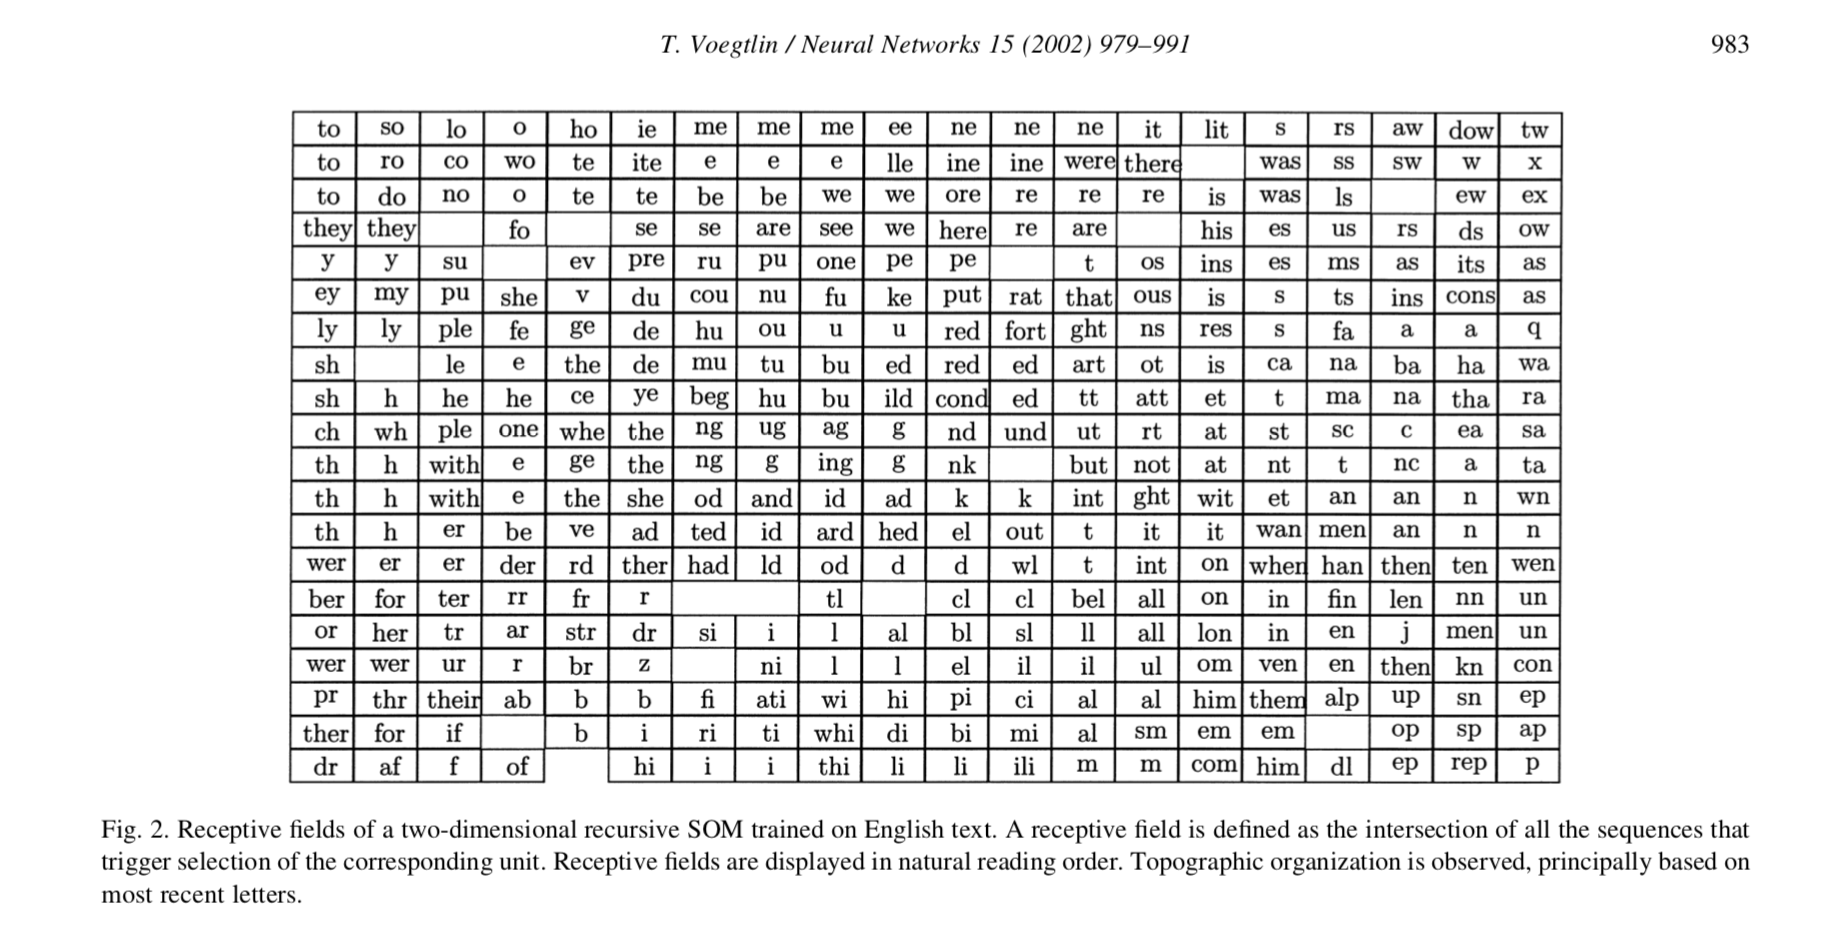
\includegraphics[width=\textwidth]{receptive_field}
\end{frame}

\begin{frame}{Progress}

\begin{itemize}
\item Read 3 articles
\item Working implementation of non-recursive SOM as base for RecSOM and mSOM implementations
\item Working implementation of simple SRN without backpropagation through time
\end{itemize}

\end{frame}


{\setbeamercolor{palette primary}{fg=black, bg=yellow}
\begin{frame}[standout]
  Questions?
\end{frame}
}

\appendix


\begin{frame}[allowframebreaks]{References}

  \bibliography{demo}
  \bibliographystyle{abbrv}
  
\begin{thebibliography}{9}
\bibitem{srn} 
Jeffrey L.Elman
\textit{Finding Structure in Time}. 
University of California, San Diego, 1990
 
\bibitem{som} 
H. Ritter and T. Kohonen
\textit{Self-Organizing Semantic Maps} 
Helsinky University of Technology, 1982
  
\bibitem{recsom} 
Thomas Voegtlin
\textit{Recursive self-organizing maps}, 2002
 
\bibitem{msom} 
Marc Strickert, Barbara Hammer
\textit{Merge SOM for temporal data}
Technical University of Clausthal, 2005
 
\end{thebibliography}

\end{frame}

\end{document}
